\subsection{Cryptographic Constructs}
\label{sec:crypto_constructs}

This section summarizes two constructs that are built on the cryptographic
primitives described in \S~\ref{sec:crypto_primitives}, and are used in the
rest of this work.


\subsubsection{Certificate Authorities}
\label{sec:certificates}

Asymmetric key cryptographic primitives assume that each party has the correct
public keys for the other parties. This assumption is critical, as the entire
security argument of an asymmetric key system rests on the fact that certain
operations can only be performed by the owners of the private keys
corresponding to the public keys. More concretely, if Eve can convince Bob
that her own public key belongs to Alice, Eve can produce message signatures
that seem to come from Alice.

The introductory material in \S~\ref{sec:crypto_primitives} assumed that each
party transmits its public key over a channel with integrity guarantees. In
practice, this is not a reasonable assumption, and the secure distribution of
public keys is still an open research problem.

The most widespread solution to the public key distribution problem is the
Certificate Authority (CA) system, which assumes the existence of a trusted
authority whose public key is securely transmitted to all the other parties in
the system.

The CA is responsible for securely obtaining the public key of each party, and
for issuing a \textit{certificate} that binds a party's identity (e.g.,
``Alice'') to its public key, as shown in Figure~\ref{fig:certificate}.

\begin{figure}[hbt]
  \centering
  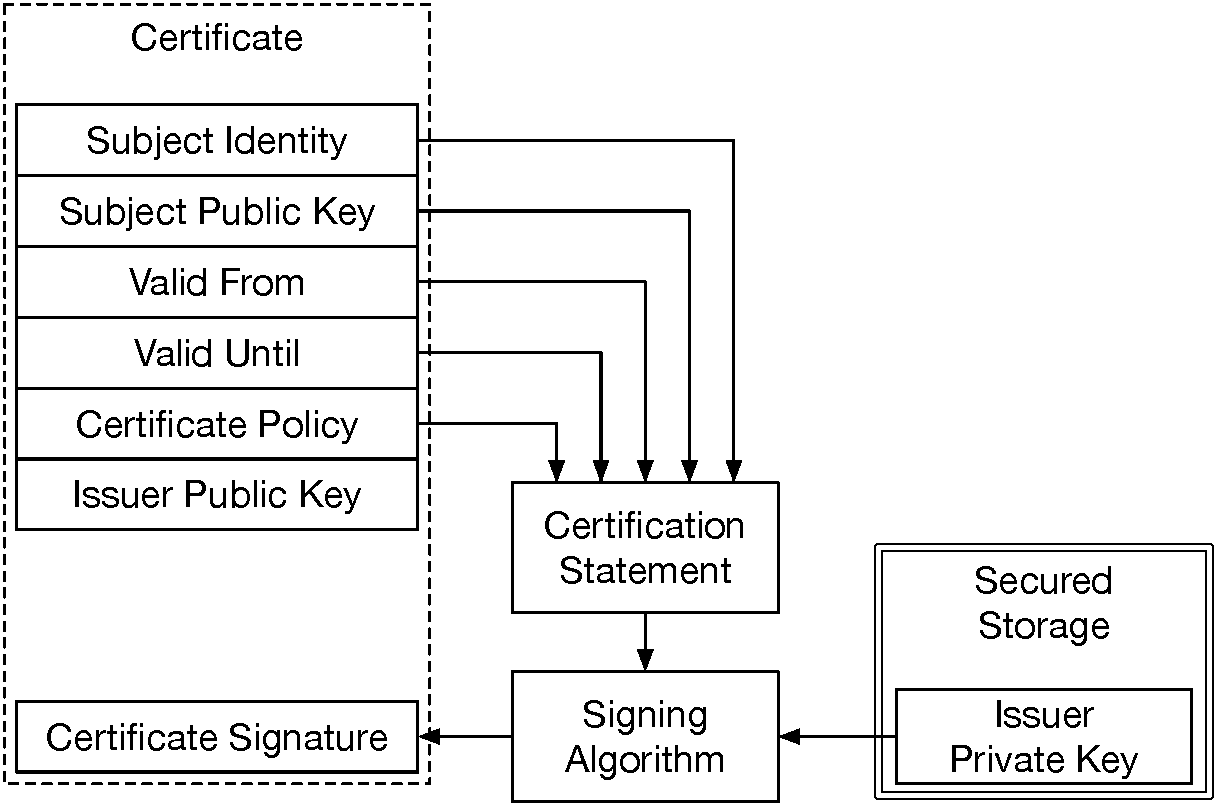
\includegraphics[width=85mm]{figures/certificate.pdf}
  \caption{
    A certificate is a statement signed by a certificate authority (issuer)
    binding the identity of a subject to a public key.
  }
  \label{fig:certificate}
\end{figure}

A certificate is essentially a cryptographic signature produced by the private
key of the certificate's \textit{issuer}, who is generally a CA. The message
signed by the issuer states that a public key belongs to a \textit{subject}.
The certificate message generally contains identifiers that state the intended
use of the certificate, such as ``the key in this certificate can only be used
to sign e-mail messages''. The certificate message usually also includes an
identifier for the issuer's \textit{certification policy}, which summarizes the
means taken by the issuer to ensure the authenticity of the subject's public
key.

A major issue in a CA system is that there is no obvious way to revoke a
certificate. A revocation mechanism is desirable to handle situations where a
party's private key is accidentally exposed, to avoid having an attacker use
the certificate to impersonate the compromised party. While advanced systems
for certificate revocation have been developed, the first line of defense
against key compromise is adding expiration dates to certificates.

In a CA system, each party presents its certificate along with its public key.
Any party that trusts the CA and has obtained the CA's public key securely can
verify any certificate using the process illustrated in
Figure~\ref{fig:certificate_validation}.

\begin{figure}[hbt]
  \centering
  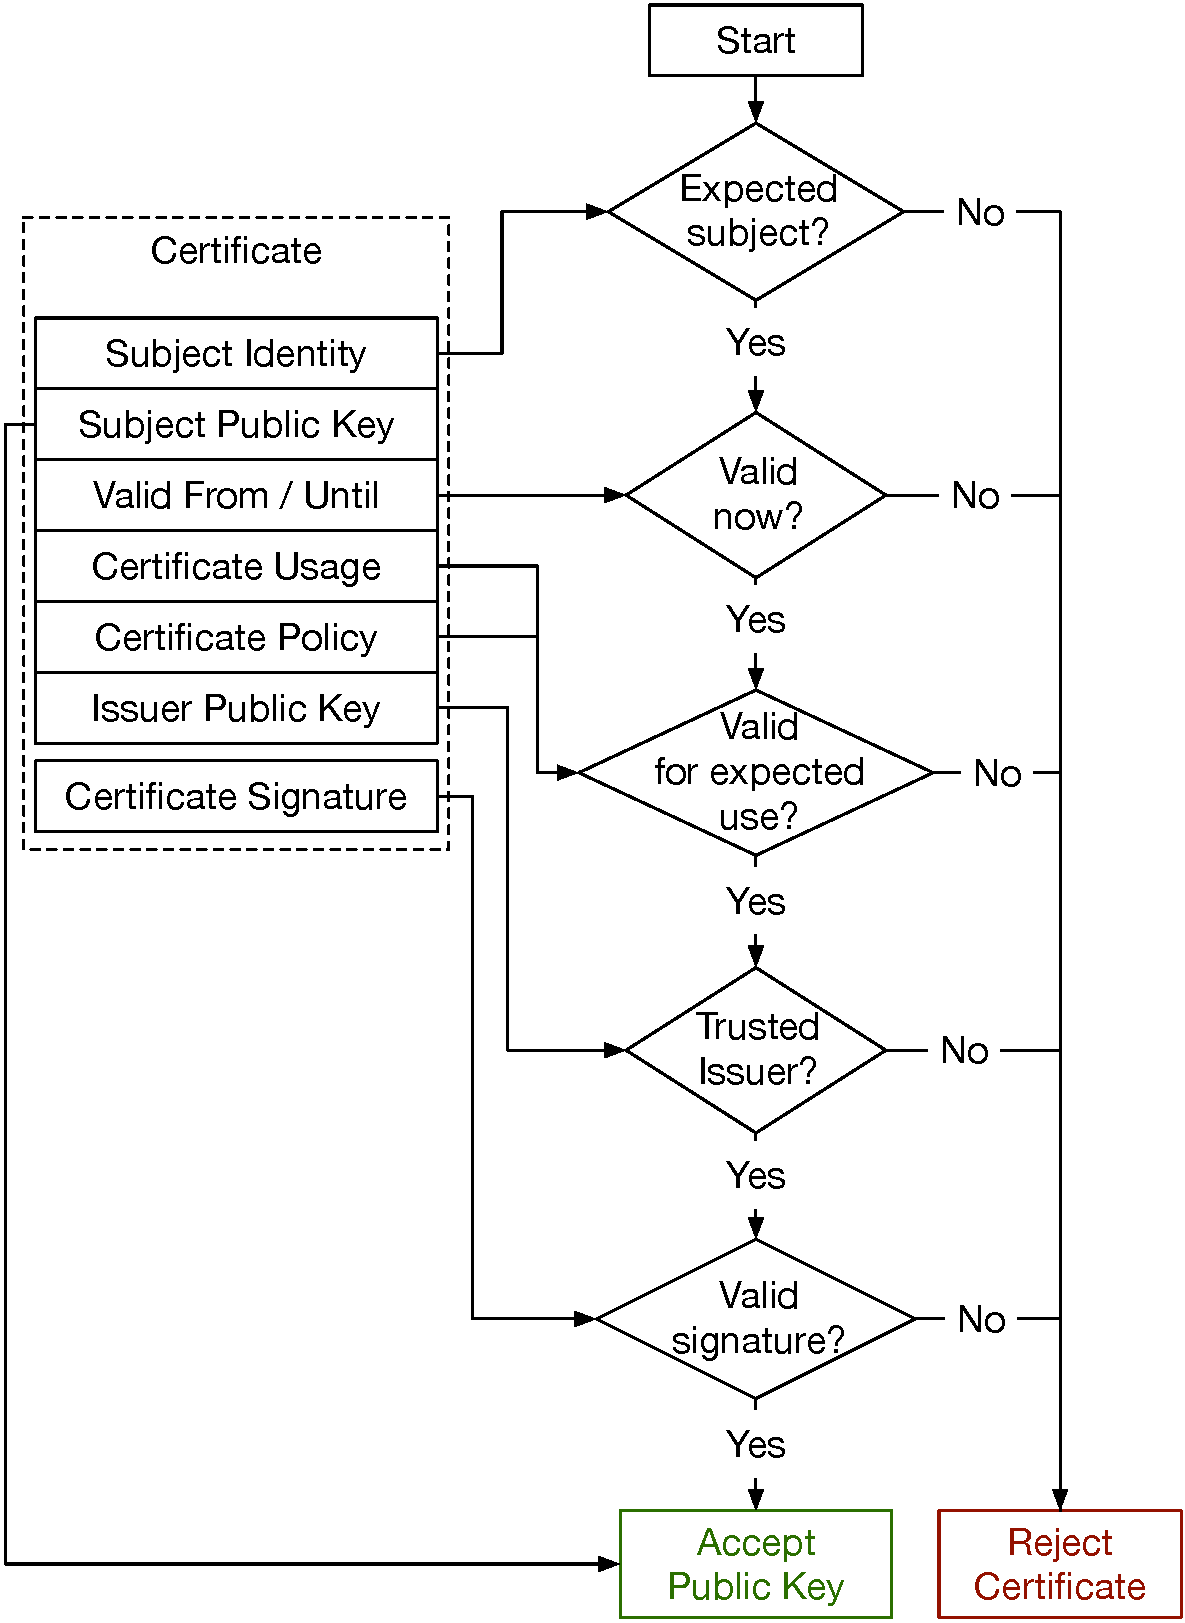
\includegraphics[width=80mm]{figures/certificate_validation.pdf}
  \caption{
    A certificate issued by a CA can be validated by any party that has
    securely obtained the CA's public key. If the certificate is valid, the
    subject public key contained within can be trusted to belong to the subject
    identified by the certificate.
  }
  \label{fig:certificate_validation}
\end{figure}

One of the main drawbacks of the CA system is that the CA's private key becomes
a very attractive attack target. This issue is somewhat mitigated by minimizing
the use of the CA's private key, which reduces the opportunities for its
compromise. The authority described above becomes the \textit{root CA}, and its
private key is only used to produce certificates for the
\textit{intermediate CAs} which, in turn, are responsible for generating
certificates for the other parties in the system, as shown in
Figure~\ref{fig:intermediate_cas}.

\begin{figure}[hbtp]
  \centering
  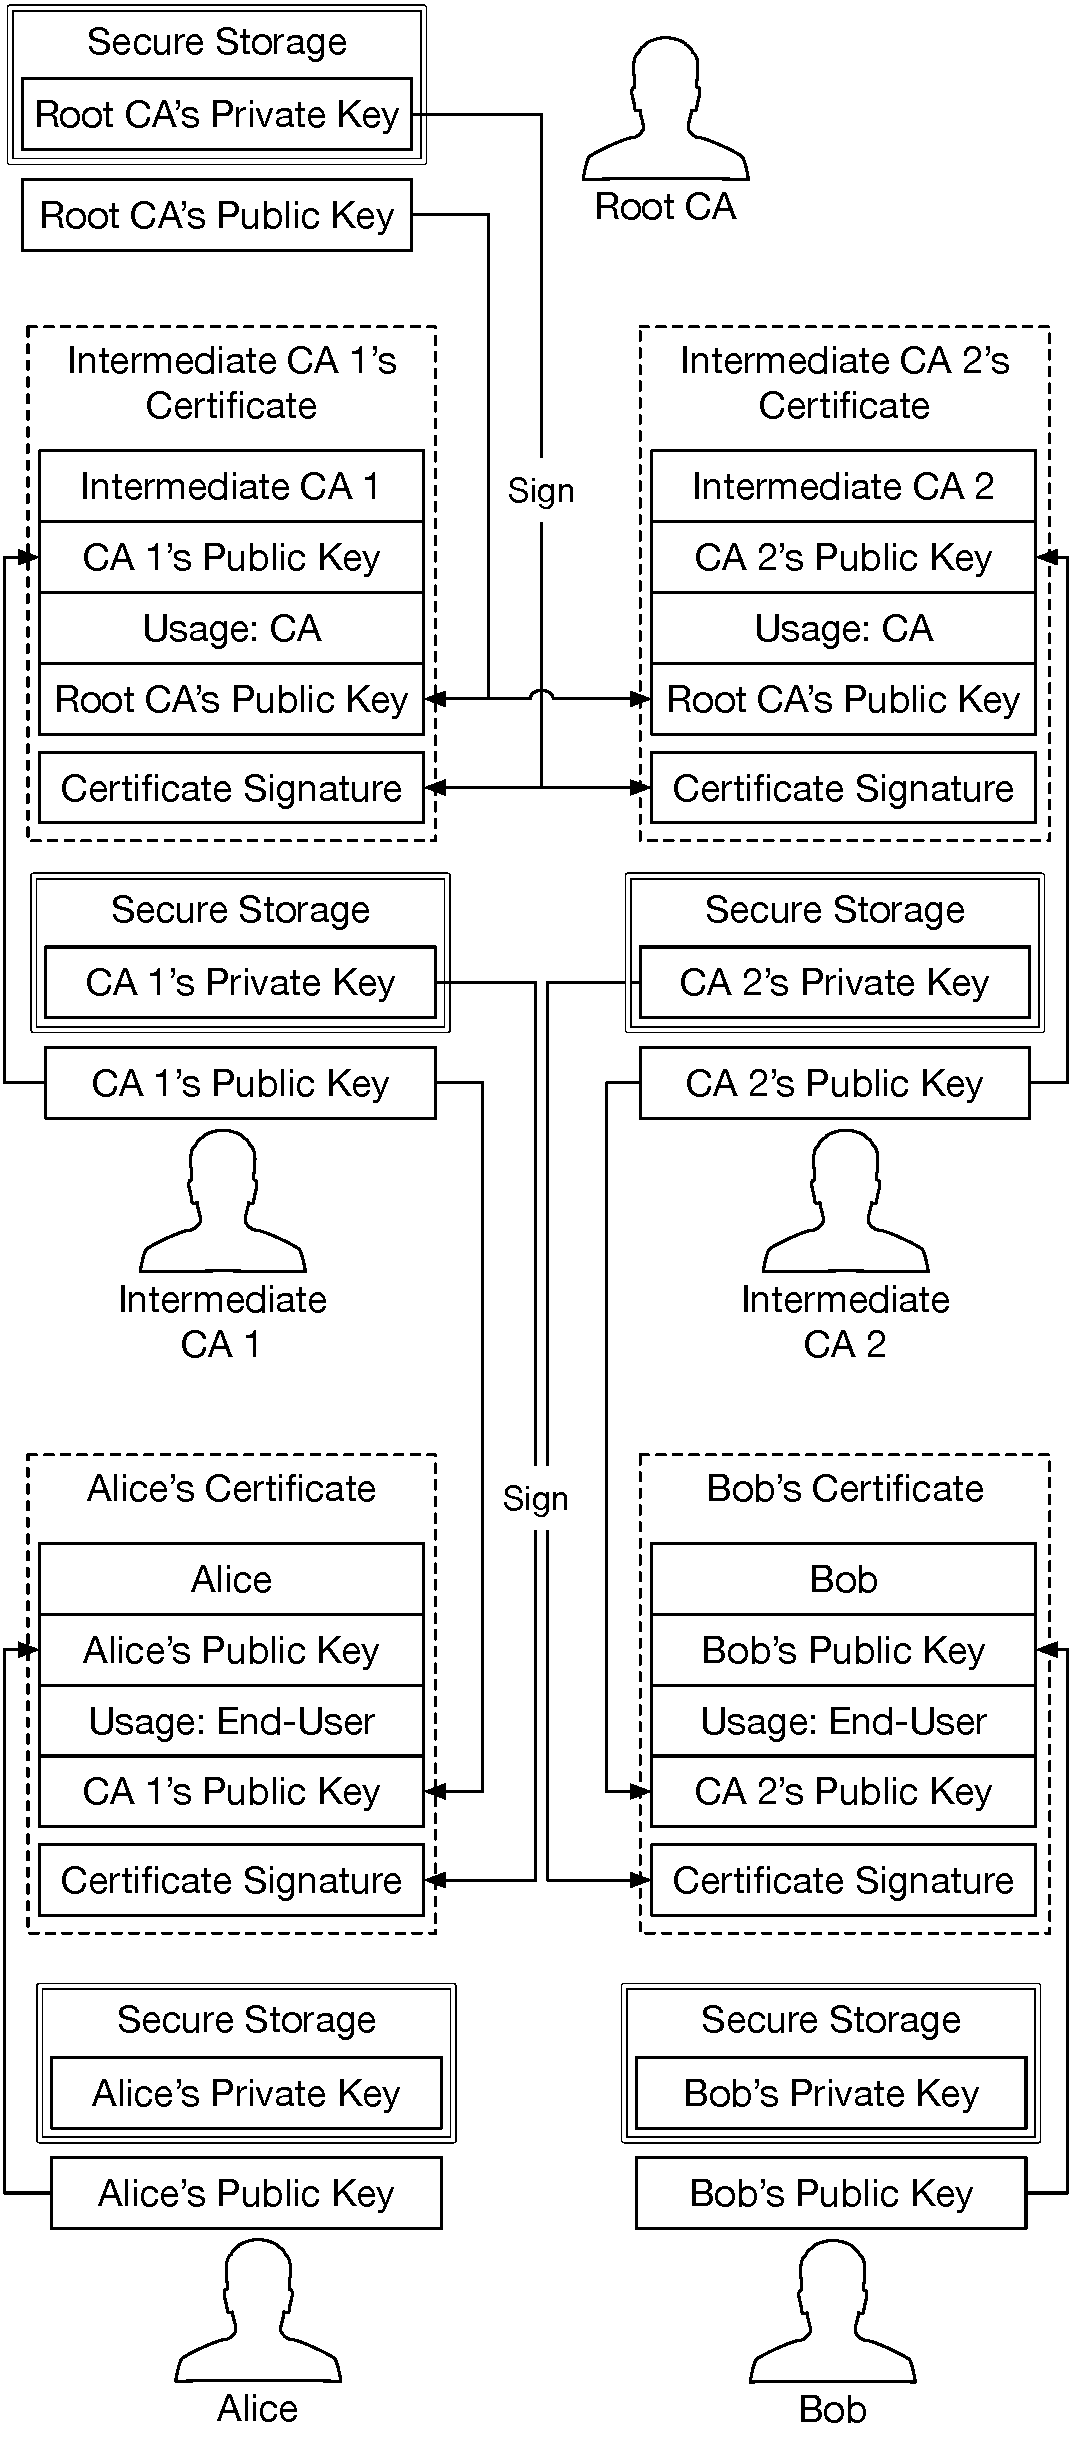
\includegraphics[width=75mm]{figures/intermediate_cas.pdf}
  \caption{
    A hierarchical CA structure minimizes the usage of the root CA's private
    key, reducing the opportunities for it to get compromised. The root CA only
    signs the certificates of intermediate CAs, which sign the end users'
    certificates.
  }
  \label{fig:intermediate_cas}
\end{figure}

In hierarchical CA systems, the only public key that gets distributed securely
to all the parties is the root CA's public key. Therefore, when two parties
wish to interact, each party must present its own certificate, as well as the
certificate of the issuing CA. For example, given the hierarchy in
Figure~\ref{fig:intermediate_cas}, Alice would prove the authenticity of her
public key to Bob by presenting her certificate, as well as the certificate of
Intermediate CA 1. Bob would first use the steps in
Figure~\ref{fig:certificate_validation} to validate Intermediate CA 1's
certificate against the root CA's public key, which would assure him of the
authenticity of Intermediate CA 1's public key. Bob would then validate Alice's
certificate using Intermediate CA 1's public key, which he now trusts.

In most countries, the government issues ID cards for its citizens, and
therefore acts as as a certificate authority. An ID card, shown in
Figure~\ref{fig:id_card_as_certificate}, is a certificate that binds a
subject's identity, which is a full legal name, to the subject's physical
appearence, which is used as a public key.

The CA system is very similar to the identity document (also known as ID card)
systems used to establish a person's identity, and a comparison between the two
may help further the reader's understanding of the concepts in the CA system.

\begin{figure}[hbt]
  \centering
  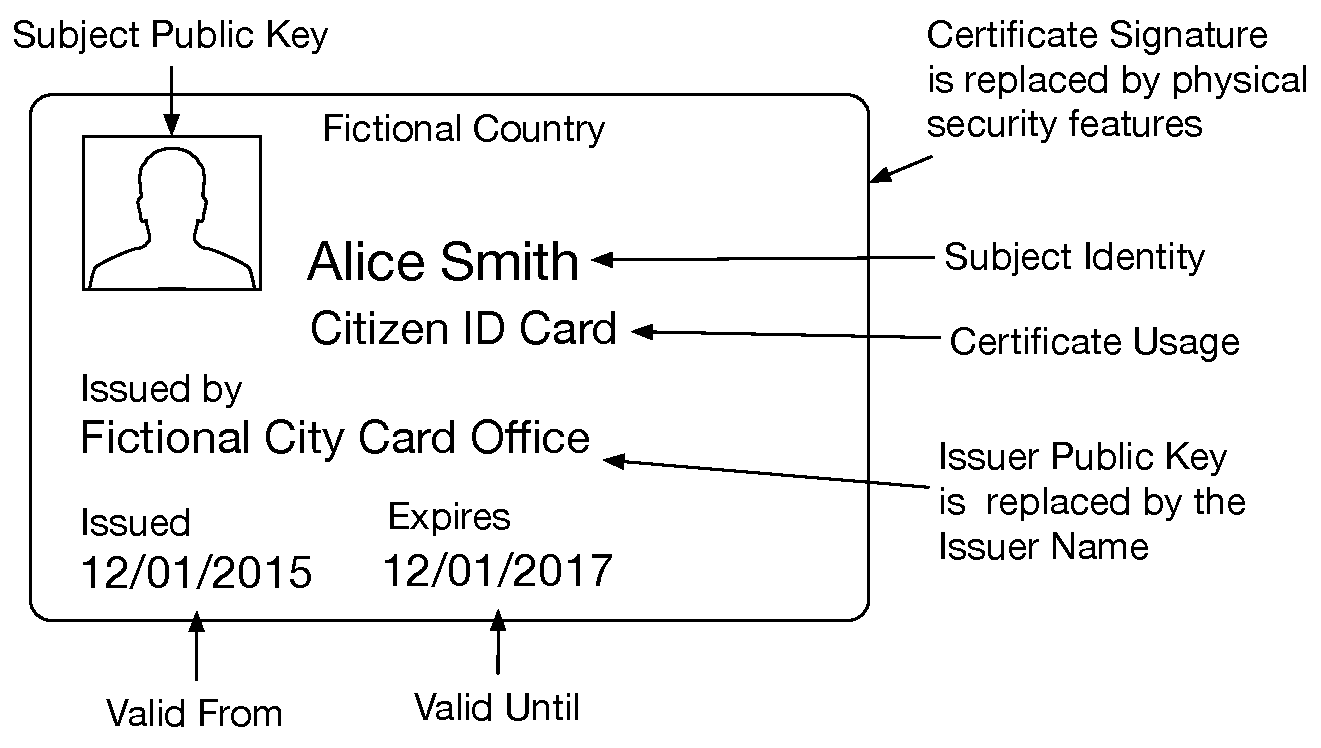
\includegraphics[width=85mm]{figures/id_card_as_certificate.pdf}
  \caption{
    An ID card is a certificate that binds a subject's full legal name
    (identity) to the subject's physical appeareance, which acts as a public
    key.
  }
  \label{fig:id_card_as_certificate}
\end{figure}

Each government's ID card issuing operations are regulared by laws, so an ID
card's issue date can be used to track down the laws that make up its
certification policy. Last, the security of ID cards does not (yet) rely on
cryptographic primitives. Instead, ID cards include physical security measures
designed to deter tampering and prevent counterfeiting .


\subsubsection{Key Agreement Protocols}
\label{sec:key_agreement}

The initial design of symmetric key primitives, introduced in
\S~\ref{sec:crypto_primitives}, assumed that when two parties wish to interact,
one party generates a secret key and shares it with the other party using a
communication channel with privacy and integrity guarantees. In practice, a
pre-existing secure communication channel is rarely available.

\textit{Key agreement protocols} are used by two parties to establish a shared
secret key, and only require a communication channel with integrity guarantees.
Figure~\ref{fig:dh_key_exchange} outlines the Diffie-Hellman Key
Exchange~(DKE)~\cite{diffie1976keyexchange} protocol, which should give the
reader an intuition for how key agreement protocols work.

\begin{figure}[hbt]
  \centering
  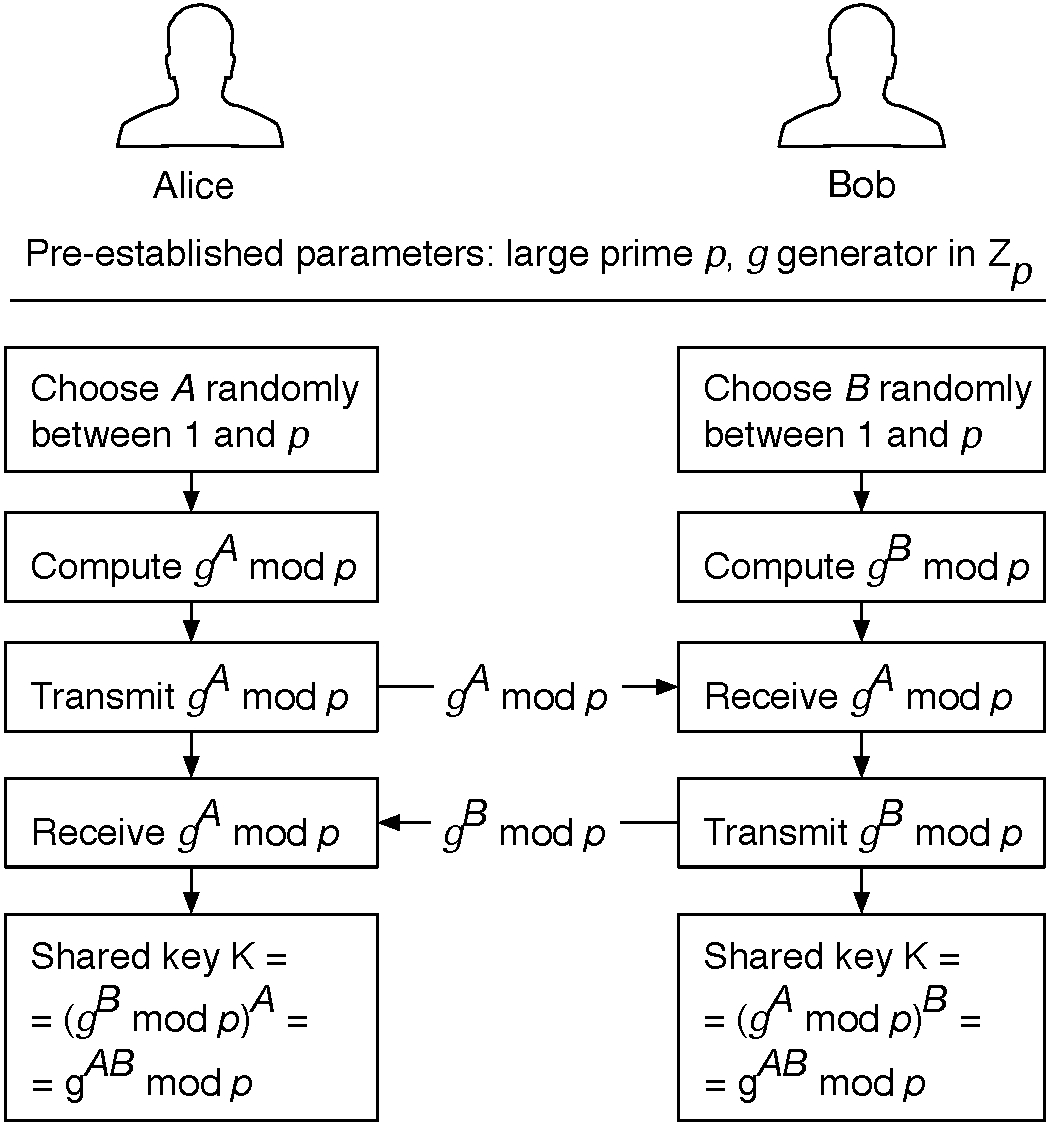
\includegraphics[width=80mm]{figures/dh_key_exchange.pdf}
  \caption{
    In the Diffie-Hellman Key Exchange (DKE) protocol, Alice and Bob
    agree on a shared secret key $K = g^{AB} \mod p$. An adversary that
    observes $g^{A} \mod p$ and $g^{B} \mod p$ cannot compute $K$.
  }
  \label{fig:dh_key_exchange}
\end{figure}

This work is interested in using key agreement protocols to build larger
systems, so we will neither explain the mathematic details in DKE, nor prove
its correctness. We note that both Alice and Bob derive the same shared secret
key, $K = g^{AB} \mod p$, without ever transmitting $K$. Furthermore, the
messages transmitted in DKE, namely $g^{A} \mod p$ and $g^{B} \mod p$, are not
sufficient for an eavesdropper Eve to determine $K$, because efficiently
solving for $x$ in $g^{x} \mod p$ is an open problem assumed to be very
difficult.

Key agreement protocols require a communication channel with integrity
guarantees. If an active adversary Eve can tamper with the messages transmitted
by Alice and Bob, she can perform a \textit{man-in-the-middle} (MITM) attack,
as illustrated in Figure~\ref{fig:key_agreement_mitm}.

\begin{figure}[hbt]
  \centering
  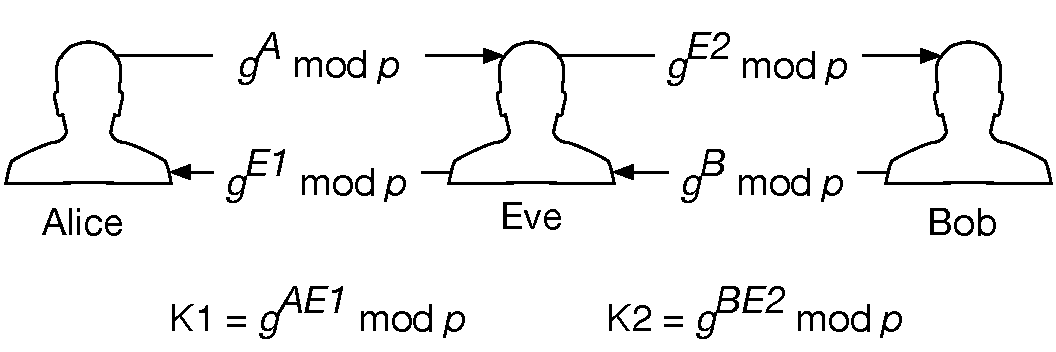
\includegraphics[width=85mm]{figures/key_agreement_mitm.pdf}
  \caption{
    Any key agreement protocol is vulnerable to a man-in-the-middle (MITM)
    attack. The active attacker performs key agreements and establishes shared
    secrets with both parties. The attacker can then forward messages between
    the victims, in order to observe their communication. The attacker can also
    send its own messages to either, impersonating the other victim.
  }
  \label{fig:key_agreement_mitm}
\end{figure}

In a MITM attack, Eve intercepts Alice's first key exchange message, and sends
Bob her own message. Eve then intercepts Bob's response and replaces it with
her own, which she sends to Alice. Eve effectively performs key exchanges with
both Alice and Bob, establishing a shared secret with each of them, without
either Bob or Alice being aware of her presence.

After establishing shared keys with both Alice and Bob, Eve can choose to
observe the communication between Alice and Bob, by forwarding messages between
them. For example, when Alice transmits a message, Eve can decrypt it using K1,
the shared key between herself and Alice. Eve can then encrypt the message with
K2, the key established between Bob and herself. While Bob still receives
Alice's message, Eve has been able to see its contents.

Furthermore, Eve can impersonate either party in the communication. For
example, Eve can create a message, encrypt it with K2, and then send it to Bob.
As Bob thinks that K2 is a shared secret key established between himself and
Alice, he will believe that Eve's message comes from Alice.

MITM attacks on key agrement protocols can be foiled by authenticating the
party who sends the last message in the protocol (in our examples, Bob) and
having it sign the key agreement messages. When a CA system is in place, Bob
uses his public key to sign the messages in the key agreement and also sends
Alice his certificate, along with the certificates for any intermediate CAs.
Alice validates Bob's certificate, ensures that the subject identified by the
certificate is who she expects (Bob), and verifies that the key agreement
messages exchanged between her and Bob match the signature provided by Bob.

In conclusion, a key agreement protocol can be used to bootstrap symmetric key
primitives from an asymmetric key signing scheme, where only one party needs to
be able to sign messages.


%\subsubsection{Cryptography for Storage}
